\section{A Complete Example}
\label{sec:complete_example}

The modules described in the previous sections of this chapter work together to
provide an adapted user interface for the sensed user's context disabilities. 
The following section presents an example which details the whole process aiming
to demonstrate the adaptation process for a concrete user interface. This 
demonstration is carried out through the introduction of particular scenario. 
This scenario introduces Molly, a user who is trying to make a phone call from 
the beach with her Android mobile device. The characteristics of Molly's context 
cause her problems to interact with the phone and achieve her goal. The main 
identified context issue is the amount of luxes in the current situation, which 
might induce temporary sight disabilities. The details of this scenario are shown
in Table~\ref{tbl:example_scenario}.

\begin{table}[H]
 \caption{Scenario summary.}
 \label{tbl:example_scenario}
 \footnotesize
 \centering
\begin{tabular}{l l}
  \hline 
				& \textbf{Scenario}	\\
  \hline
  User \\
  \qquad - Personal data 	& Molly, $39$ years old, United States\\
  \qquad - Activity	 	& Phone call		\\
  \qquad - Known disabilities 	& - 			\\
% 				& Hearing loss 		\\
%   \hline
  Context \\
  \qquad - Location 		& Relative: Plentzia, Spain\\
				& 			\\
  \qquad - Time			& $14$:$35$ 		\\
  \qquad - Brightness		& $30,000$ \ac{lx}	\\
  \qquad - Noise		& $80$ \acp{db}		\\
  \qquad - Temperature		& $28$ ºC 		\\
%   \hline
  Device 			& Samsung Galaxy SII 	\\
				& Battery: $55$\%	\\
  \hline
\end{tabular}
\end{table}

% The following lines detail the adaptation process, highlighting each layer's and
% module's goal and behaviour. As the user is trying to perform a phone call, the 
% corresponding default user interface is shown in Figure~\ref{fig:example_scenario_default}.

To make the phone call, Molly is using the application whose user interface is
shown in Figure~\ref{fig:example_scenario_default}. Thus, the shown user interface
should be adapted by AdaptUI if the scenario presents characteristics that might
trouble Molly during the phone call process.

\begin{figure}[H]
\centering
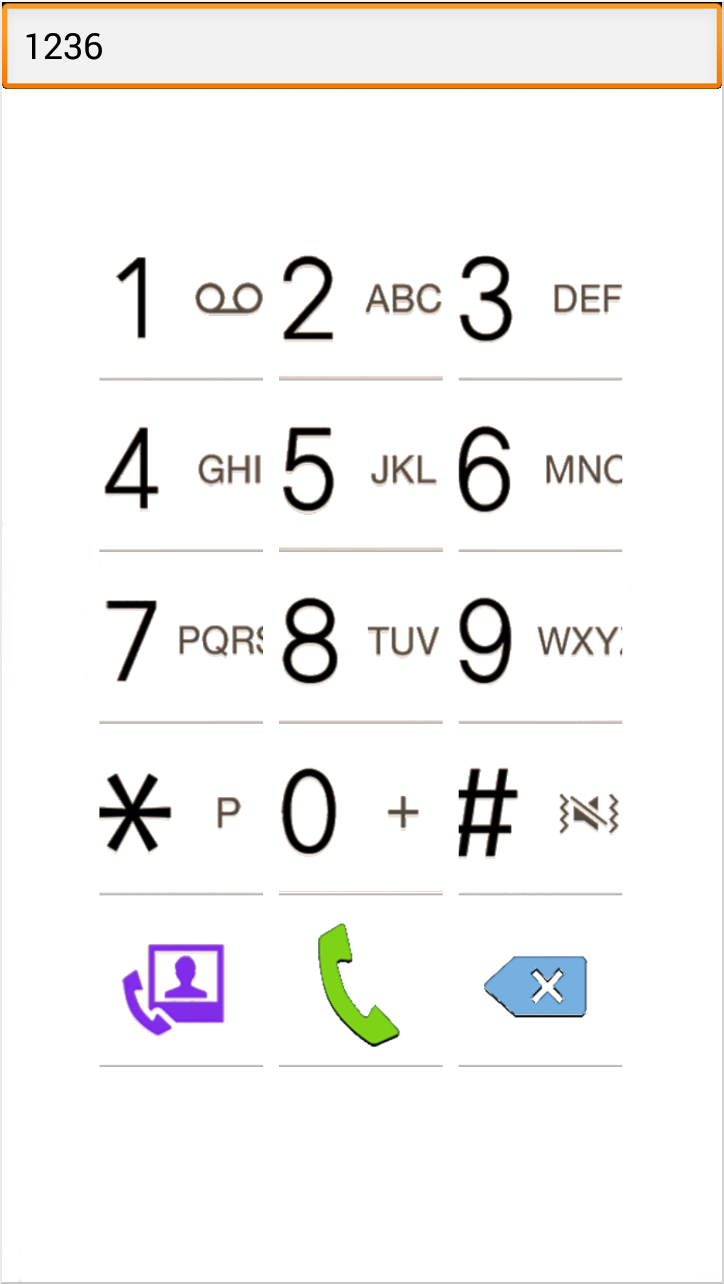
\includegraphics[width=0.35\textwidth]{example_scenario_default.png}
\caption{A simple phone call application user interface.}
\label{fig:example_scenario_default}
\end{figure}

First, the proper functioning of the AdaptUI platform highly depends on the
interaction capabilities represented in the AdaptUIOnt ontology. These capabilities
are first gathered by the Capabilities Collector. This module also collects context
and device characteristics to build the corresponding semantic model. Hence,
the Capabilities Collector has to be run by Molly in her device. The first task
this module performs is collecting several characteristics of the used device.
This is made by calling several Android system methods which allow developers
know the current capabilities of the device (e.g., available memory and battery).
Next, several activities are presented through which Molly is asked to calibrate
and configure different visual elements, such as buttons, edit texts and text
views. This has to be performed considering the current context situation. 
Otherwise, it would not be useful for future adaptations within a similar context. 
As the context might vary during the capabilities collecting process, the module
uses a native pre-semantic representation of the gathered knowledge. Using a simple
key-value representation each interaction is stored in a SharedPreferences based
model. This allows Molly to specify the needed interaction preferences rapidly.
The process ends with the translation of this model into a semantic one, represented
by the AdaptUIOnt ontology. This takes several seconds, and it is performed by
the Semantic Modeller. Taking into account the characteristics of the scenario 
presented in Table~\ref{tbl:example_scenario}, Molly specifies the following
interaction features:
% 
% \begin{itemize}
%   \item From the interface point of view, Molly does not change the interaction
%   input or output system.
%   \item 
% \end{itemize}


\begin{itemize}
%%%%%%%%%%%%%%%%%%%%%%%%%%%%%%%%%%%%%%%%%%%%%%%%%%%%%%%%%%%%%%%%%%%%%%%%%%%%%%%%
%%%%%%%%%%%%%%%%%%%%%%%%%%Modelling Layer%%%%%%%%%%%%%%%%%%%%%%%%%%%%%%%%%%%%%%%
%%%%%%%%%%%%%%%%%%%%%%%%%%%%%%%%%%%%%%%%%%%%%%%%%%%%%%%%%%%%%%%%%%%%%%%%%%%%%%%%
  \item The Modelling Layer aims to build a semantic model of the user, context
  and device, based on the interaction characteristics available in the current
  situation. For further details of the Modelling Layer see Section~\ref{sec:modelling_layer}.
  
  \begin{itemize}
    %Capabilities Collector%%%%%%%%%%%%%%%%%%%%%%%%%%%%%%%%%%%%%%%%%%%%%%%%%%%%%
    \item First, the user has to use the Capabilities Collector. As explained in 
    Section~\ref{sec:capabilities_collector}, this software module collects non 
    physiological capabilities of the user, gathers different variables of the 
    current context, and identifies several device characteristics. An example of 
    the Capabilities Collector is given through 
    Figure~\ref{fig:capabilities_collector_scenario}. Through a series of
    activities, the user is requested to dynamically configure different user 
    interface components taking into account the current scenario characteristics. 
    Each activity presents different user interface views, and the user's
    interaction decisions are stored in an Android SharedPreferences model.
    This model is easy to maintain and manipulate, and it serves as input for
    the next module. The user, context and device profiles are detailed in 
    Table~\ref{tbl:profiles}.
    
\begin{figure}
\centering
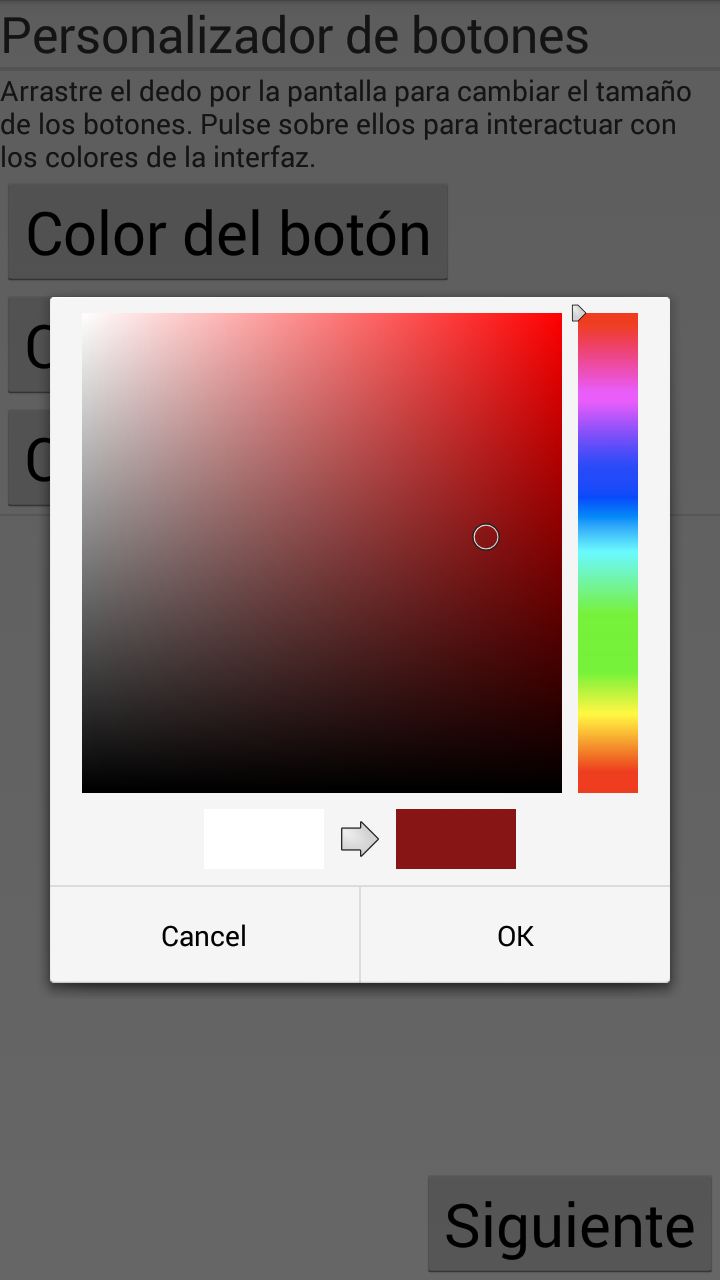
\includegraphics[width=0.35\textwidth]{capabilities_collector_scenario.png}
\caption{A user configuring the buttons colour set through the Capabilities Collector.}
\label{fig:capabilities_collector_scenario}
\end{figure}
    
\begin{table}
 \caption{User, context and device profiles after using the Capabilities Collector.
 The class (*) is translated to a semantic representation in the AdaptUIOnt ontology.
 It is not represented in the SharedPreferences model. The colour set (*) represents
 the whole colour configuration that the user specifies for the corresponding
 views, including the background colours, text colours and so on.}
 \label{tbl:profiles}
 \footnotesize
 \centering
\begin{tabular}{l l l l}
  \hline 
  \textbf{Entity}& \textbf{Class(*)}& \textbf{SharedPreferences} & \textbf{Value}\\
		& 		& \textbf{property} 		& \\
  \hline
  User 		& Interface 	& \textit{input}		& default	\\
		& 		& \textit{output} 		& default	\\
		& View		& \textit{colourSet(*)}		& default	\\
		& Display 	& \textit{minBrightness}	& $9$		\\ 
		& 		& \textit{maxBrightness}	& max		\\
		& Audio 	& \textit{minVolume}		& $4$		\\
		& 		& \textit{maxVolume} 		& max		\\
		& Other 	& \textit{language}		& English	\\
		& 		& \textit{vibration} 		& true 		\\
		
  Context	& Brightness	& \textit{brightness}		& $30,000$	\\
		& Noise		& \textit{noise}		& $80$		\\
		& Time		& \textit{time}			& $14$:$35$	\\
		& Location	& \textit{city}			& Plentzia	\\
		&		& \textit{country}		& Spain		\\
		&		& \textit{longitude}		& $43.414353$	\\
		&		& \textit{latitude} 		& $-2.944183$	\\
  Device	& \ac{os}	& \textit{osVersion}		& $4.1.2$	\\
		& Battery	& \textit{battery}		& $55$		\\
		& Volume	& \textit{maxVolume}		& $12$		\\
		& Brightness	& \textit{maxBrightness}	& $15$		\\
		& DeviceScreenResolution & \textit{resolution}	& $480×800$	\\	
  \hline
\end{tabular}
\end{table}

    %Semantic Modeller%%%%%%%%%%%%%%%%%%%%%%%%%%%%%%%%%%%%%%%%%%%%%%%%%%%%%%%%%%
    \item Once the interaction with the Capabilities Collector is finished, the
    Semantic Modeller (see Section~\ref{sec:semantic_modeller}) uses the 
    SharedPreferences stored model and stores it as a semantic representation of 
    this model in the AdaptUIOnt ontology. This is performed thanks to the 
    \textit{Pellet4Android} mobile semantic engine, which allows to manipulate 
    semantic knowledge in Android. Storing in the ontology requires more time 
    than using SharedPreferences. Thus, the last operation in the Modelling Layer 
    is the semantic storage. The most significant represented characteristics 
    are shown in Table~\ref{tbl:capabilities_collector_scenario}. Those 
    characteristics that are not present in Table~\ref{tbl:profiles} are computed 
    by the pre-adaptation. For example, Equation~\ref{ec:pre_rule_1} updates the 
    \textit{userAuxDisplayHasApplicable} datatype property by checking if the 
    user interacts with the Capabilities Collector in a \textit{default} manner.
    
    \footnotesize
    \begin{equation} \label{ec:pre_rule_1} 
    \begin{align*} 
    adaptui:UserAux(?uaux) ∧ adaptui:UserCharacteristics(?user) ∧ \\
    adaptui:Interface(?interf) ∧ adaptui:Input(?input) ∧ \\
    userHasInterface(?user, ?interf) ∧ interfaceHasInput(?interf, ?input) ∧\\
    swrlb:equal("default") \\    
    \Rightarrow \\
    adaptui:userAuxDisplayHasApplicable(?uaux, true)
    \end{align*}
    \end{equation}
    \normalsize
    
    

  \end{itemize}

\begin{table}
 \caption{User, context and device profiles as represented in the AdaptUIOnt ontology.}
 \label{tbl:capabilities_collector_scenario}
 \footnotesize
 \centering
\begin{tabular}{l l l l}
  \hline 
  \textbf{Entity}& \textbf{Class} & \textbf{Property} 			& \textbf{Value}\\
  \hline
  User 		& Display 	& \textit{userDisplayIsApplicable} 	& true		\\% Esto se saca con reglas
		& 		& \textit{userDisplayBrightnessIsStatic}& false		\\
		& Audio 	& \textit{userDisplayApplicableIsStatic}& false		\\
		& 		& \textit{userAudioHasApplicable} 	& true		\\
		& 		& \textit{userAudioApplicableIsStatic} 	& false		\\
		& 		& \textit{userAudioHasVolume}  		& $4$ 		\\
		& Interface 	& \textit{userInterfaceInput}		& default	\\
		& 		& \textit{userInterfaceOutput} 		& default	\\
% 		& Experience	& \textit{userHasExperience} 		& high		\\
		& View		& \textit{userViewIsStatic}		& false		\\
		& Other 	& \textit{userHasLanguage}		& English	\\
		& 		& \textit{vibration} 			& true 		\\
  Context	& Brightness	& \textit{contextHasBrightness}		& $30,000$	\\
		& Noise		& \textit{contextHasNoise}		& $80$		\\
		& Time		& \textit{contextHasTime}		& $14$:$35$	\\
		& Location	& \textit{contextHasRelativeLocationCity}& Plentzia	\\
		&		& \textit{contextHasRelativeLocationCountry}& Spain	\\
		&		& \textit{contextHasAbsoluteLocationLongitude}& $43.414353$\\
		&		& \textit{contextHasAbsoluteLocationLatitude} & $-2.944183$\\
  Device	& Software (\ac{os})& \textit{deviceHasOSVersion}	& $4.1.2$	\\
		& Hardware (Battery)& \textit{deviceHasBattery}		& $55$		\\
		& (Volume)	& \textit{deviceHasMaxVolume}		& $12$		\\
		& (DeviceScreenResolution) & \textit{deviceHasResolution}& $480×800$	\\	
  \hline
\end{tabular}
\end{table}

%%%%%%%%%%%%%%%%%%%%%%%%%%%%%%%%%%%%%%%%%%%%%%%%%%%%%%%%%%%%%%%%%%%%%%%%%%%%%%%%
%%%%%%%%%%%%%%%%%%%%%%%%%%Adaptation Layer%%%%%%%%%%%%%%%%%%%%%%%%%%%%%%%%%%%%%%
%%%%%%%%%%%%%%%%%%%%%%%%%%%%%%%%%%%%%%%%%%%%%%%%%%%%%%%%%%%%%%%%%%%%%%%%%%%%%%%%
  \item After storing the semantic model in the AdaptUIOnt ontology, it is sent
  to the the Adaptation Layer. This layer aims to lead the dynamic adaptation of
  the elements presented in the user interface.
  
  \begin{itemize}
    %Adaptation Engine%%%%%%%%%%%%%%%%%%%%%%%%%%%%%%%%%%%%%%%%%%%%%%%%%%%%%%%%%%
    \item The Adaptation Engine loads, as input, the stored AdaptUIOnt model, 
    and it executes the corresponding adaptation rules defined by the developer. 
    Once the rules have been executed, the resulting user interface is dynamically 
    updated and presented to the user. Equation~\ref{ec:adap_rule_8} shows how
    the views are updated due to the context brightness. The resulting adapted
    user interface is shown in Figure~\ref{fig:example_scenario_default_vs_adapted}.

    \footnotesize
    \begin{equation} \label{ec:adap_rule_8} 
    \begin{align*} 
    adaptui:Button(?b) ∧ adaptui:ContextCharacteristics(?c) ∧ gumo:Light(?light) ∧ \\  
    gumo:PhysicalEnvironment(?pe) ∧ contextHasPhysicalEnvironment(?c, ?pe) ∧ \\ 
    lightHasBrightness(?light, ?value) ∧ physicalEnvironmentHasLight(?pe, ?light) ∧ \\
    swrlb:greaterThanOrEqual(?value, 20000) \\
    \Rightarrow \\
    adaptui:buttonHasBackgroundColor(?b, -16711936)
    \end{align*}
    \end{equation}
    \normalsize
    
    \begin{figure}
    \centering
    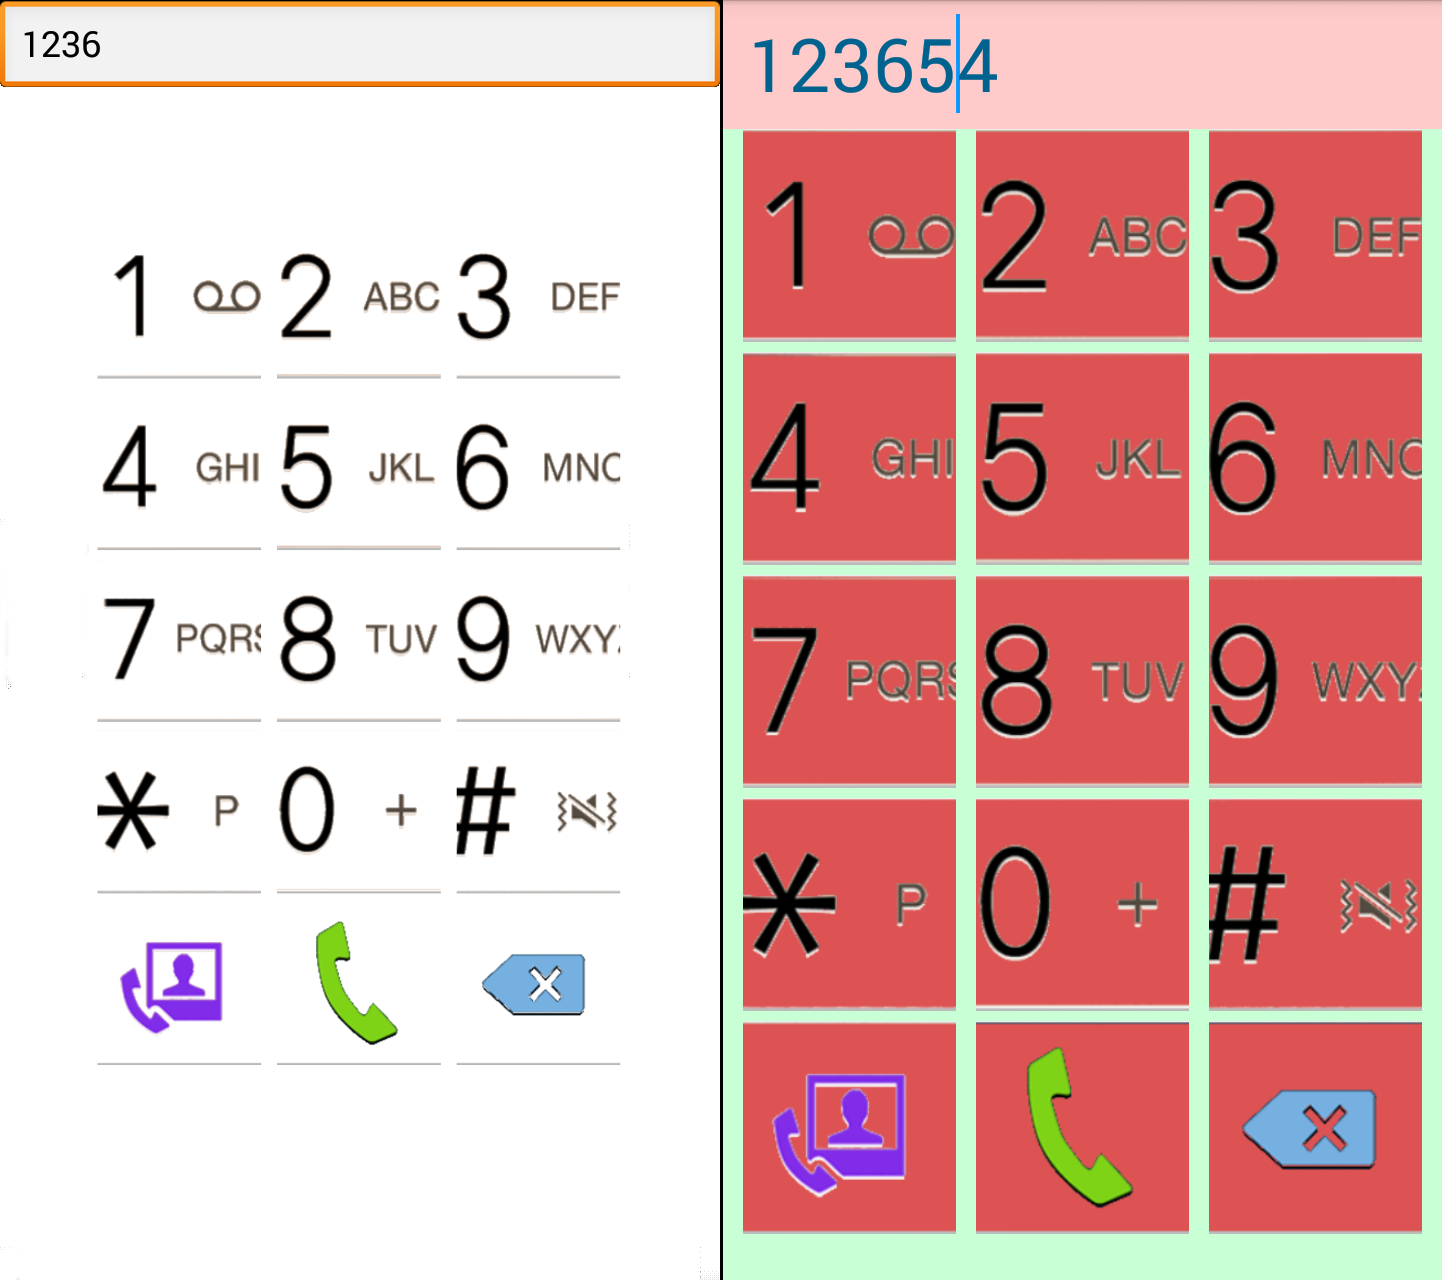
\includegraphics[width=0.50\textwidth]{example_scenario_default_vs_adapted.png}
    \caption{The default user interface (left) and the adapted user interface (right).}
    \label{fig:example_scenario_default_vs_adapted}
    \end{figure}
    
    %Adaptation Polisher%%%%%%%%%%%%%%%%%%%%%%%%%%%%%%%%%%%%%%%%%%%%%%%%%%%%%%%%
    \item Finally, the Adaptation Polisher monitors the usability of the adapted
    user interface. To safeguard this usability it builds and compares two
    interaction models. The first one is built with the usability metrics detailed
    in Section~\ref{sec:usability_metrics} under default circumstances. This means
    that this model is fully accessible by the user in many contexts. The second 
    model, is built from the same usability metrics but taking into account the 
    adapted user interface. The Interaction Model Comparator executes the following
    interaction rules, which aim to evaluate the usability metrics differences
    between the two interaction models. Once these rules are executed, their
    results update the last adaptation of the user interface if needed. The
    polished user interface is compared with the adapted one in 
    Figure~\ref{fig:example_scenario_adapted_vs_polished}. In the presented
    scenario, the Equation~\ref{ec:pre_rule_8} updates polishes the button's
    text as follows: 

    \footnotesize
    \begin{equation} \label{ec:pre_rule_8} 
    \begin{align*} 
    adaptui:Button(?b) ∧ adaptui:Usability (?u) ∧ adaptui:EfficiencyMetric(?em) ∧ \\
    usabilityHasEfficiencyMetric(?u, ?em) ∧ swrlb:greaterThanOrEqual(?value, 0.5) ∧ \\
    efficiencyMetricHasTaskEffectiveness(?em, ?value)\\
    \Rightarrow \\
    adaptui:buttonHasTextColor(?b, 16777215)
    \end{align*}
    \end{equation}
    \normalsize

    \begin{figure}
    \centering
    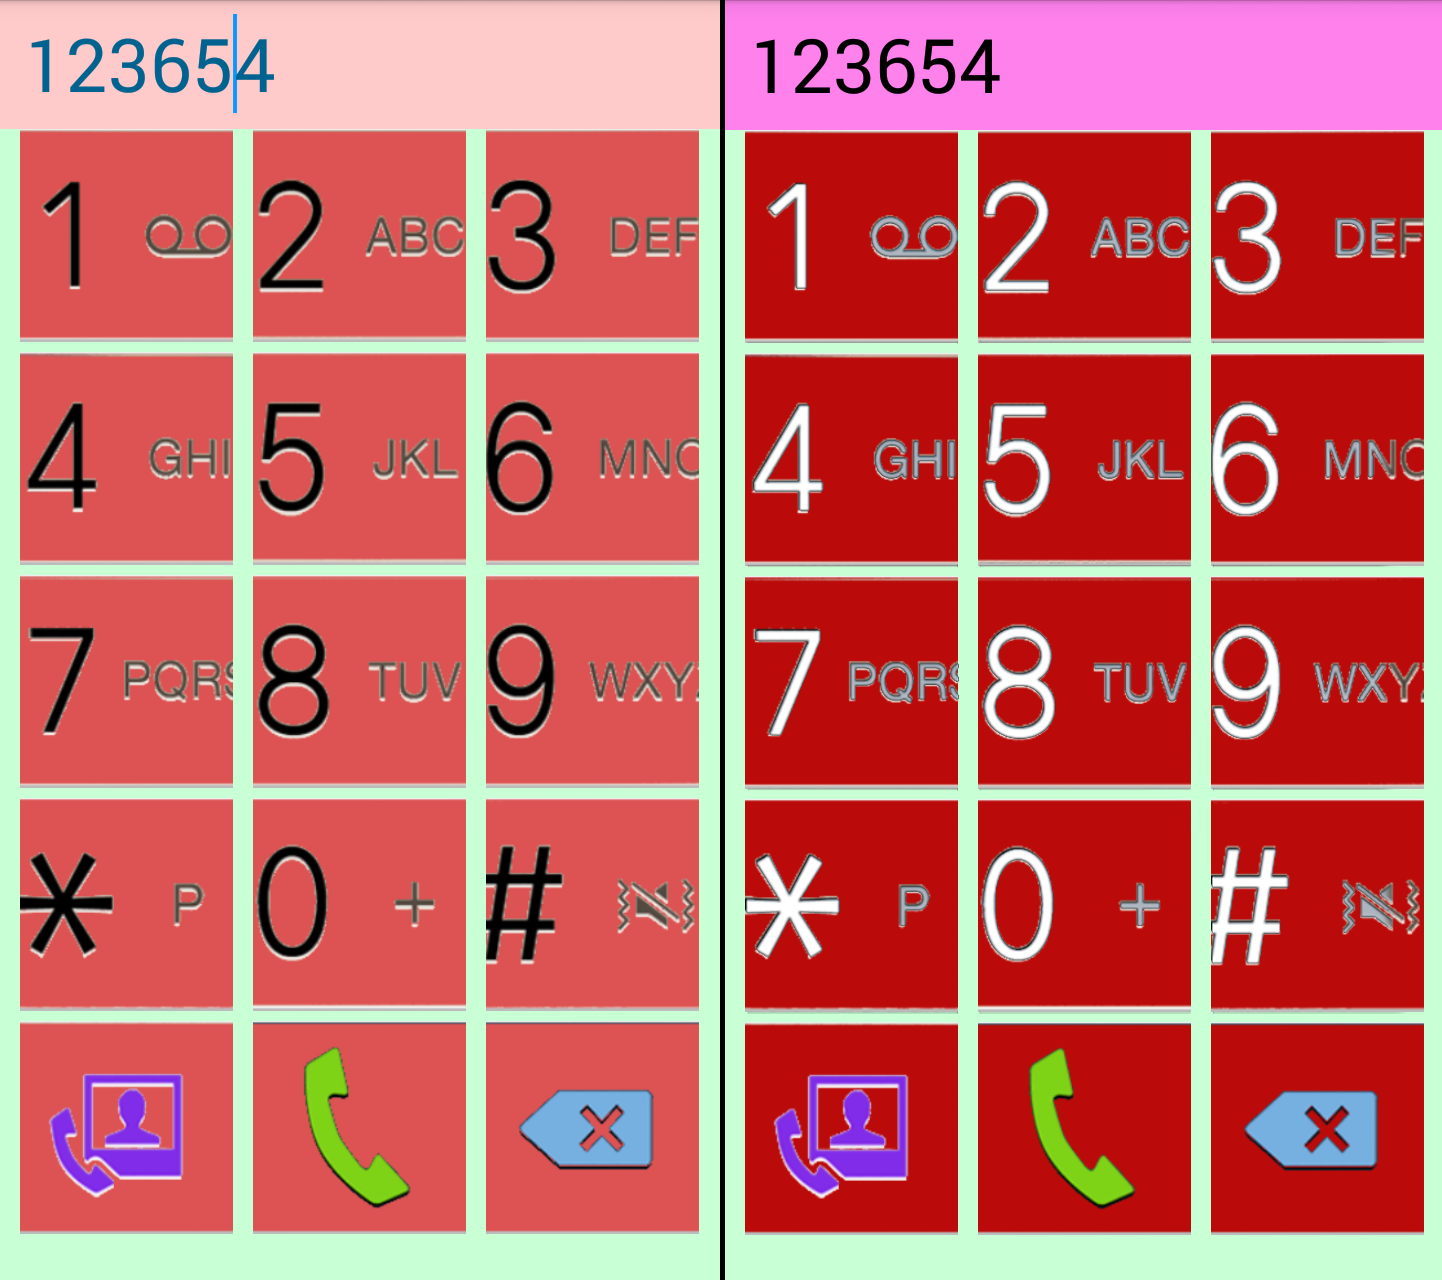
\includegraphics[width=0.50\textwidth]{example_scenario_adapted_vs_polished.png}
    \caption{The adapted user interface (left) and the polished user interface (right).}
    \label{fig:example_scenario_adapted_vs_polished}
    \end{figure}

  \end{itemize}

\end{itemize}

As this example demonstrates, the polisher rules allow the developer to keep
improving the adapted user interfaces. This is carried out by maintaining both
default and adapted interaction models which are based on the usability metrics
detailed in Section~\ref{sec:usability_metrics}.

% Modelling Layer
% - Capabilities Collector
% 1. Llegan las capacidades.
% 2. Se genera el modelo.
% 3. Se guarda en formato SharedPreferences.
% - Semantic Layer
% 4. Se guarda en formato semántico.
% 
% Adaptation Layer
% - Adaptation Engine
% 1. Se analiza el modelo semántico.
% 2. Se ejecutan las reglas correspondientes.
% 3. Se actualiza la interfaz con la nueva adaptación resultante.
% - Adaptation Polisher
% 1. Se genera el modelo de interacción.
% 2. Se ejecutan las reglas de interacción.
% 3. Se envían los resultados al Polishing instructions Generator.
% 4. Se ejecutan las reglas de polishing.
% 5. Se envía al Adaptation Engine la interfaz a adaptar.
